\documentclass[24pt,pdf,hyperref={unicode}]{beamer}
\usepackage[utf8]{inputenc}
\usepackage{aiml}
\usetikzlibrary{calc}
\usetikzlibrary{shapes.geometric}

\begin{document}

\begin{frame}
\uncover<+->{$$
n(x_1,\ldots,x_n)=f\left(\sum_{i=1}^n x_iw_i\right)
$$}
\uncover<+->{$$
n(x_1,x_2)=x_1x_2?
$$}
\only<+>{$$
\begin{tikzpicture}[x=3cm]
\node[neu] (n) at (0,0) {$f(x)=x$};
\node (x) at (-1,0) {$x_1$};
\path (x) edge[->] node[above]{$x_2$} (n);
\node (y) at (1,0) {$x_1x_2$};
\path (n) edge[->] (y);
\end{tikzpicture}
$$}
\uncover<+->{$$
x_1x_2=\exp(\ln x_1 + \ln x_2)
$$}
\uncover<+->{$$
\begin{tikzpicture}[x=1.5cm]
\node (x1) at (0,1) {$x_1$};
\node (x2) at (0,-1) {$x_2$};
\node[neu] (n1) at (1,1) {$\ln$};
\node[neu] (n2) at (1,-1) {$\ln$};
\path (x1) edge[->] node[above] {$1$} (n1);
\path (x2) edge[->] node[above] {$1$} (n2);
\node[neu] (n3) at (2,0) {$\exp$};
\path (n1) edge[->] node[above] {$1$} (n3);
\path (n2) edge[->] node[above] {$1$} (n3);
\node (y) at (3,0) {$x_1x_2$};
\path (n3) edge[->] (y);
\end{tikzpicture}
$$}

\end{frame}


\begin{frame}
\bio{Hilbert}{David Hilbert}{Mathematische Probleme (1900)}
\end{frame}

\begin{frame}
Тринадцатая проблема Гильберта:\\[1cm]

Можно ли решить общее уравнение седьмой степени с помощью функций, зависящих только от двух переменных?
\end{frame}

\begin{frame}
\begin{small}
\doublebio
{Arnold}{Владимир Игоревич Арнольд}
{Kolmogorov}{Андрей Николаевич Колмогоров}
{
$ $\\[0.2cm]

О представлении непрерывных функций трех переменных суперпозициями непрерывных функций двух переменных (1959)\\[0.2cm]

О представлении непрерывных функций нескольких переменных в виде суперпозиций непрерывных функций одной переменной и сложения (1957)}
\end{small}
\end{frame}

\begin{frame}

$$
f(x_1,\dots,x_n)=\sum_{q=0}^{2 n} \Phi_q \left(\sum_{p=1}^n\psi_{q,p}(x_p)\right)
$$
\end{frame}

\begin{frame}\frametitle{Сеть Эльмана}
\begin{center}
\begin{tikzpicture}[x=2cm,y=-2cm]
\node (x) at (0,0) {X};
\node (c) at (1,1) {C};
\node[neu] (h) at (2,0) {H};
\node[neu] (o) at (3,0) {O};
\node  (y) at (4,0) {Y};
\path (x) edge[->] (h);
\path (c.east) edge[->] (h.south west);
\path (h) edge[->] (o);
\path (o) edge[->] (y);
\draw[->] ($(h.east)+(0.1,0)$) |- ($(c)+(-0.6,0.5)$) |- (c.west);
\end{tikzpicture}
\end{center}
\end{frame}

\begin{frame}\frametitle{Сеть Эльмана}
\begin{center}
\begin{tikzpicture}[x=2cm,y=-2cm]
\node (x) at (0,0) {\{0,1\}};
\node (c) at (1,1) {c};
\node[neu] (h) at (2,0) {+};
\node[neu] (o) at (3,0) {e};
\node  (y) at (4,0) {Y};
\path (x) edge[->] (h);
\path (c.east) edge[->] (h.south west);
\path (h) edge[->] (o);
\path (o) edge[->] (y);
\draw[->] ($(h.east)+(0.1,0)$) |- ($(c)+(-0.6,0.5)$) |- (c.west);
\end{tikzpicture}
\end{center}
\end{frame}

\begin{frame}\frametitle{Обучение рекуррентных сетей}

\begin{tikzpicture}[x=2cm,y=-2cm]
\node (x) at (0,0) {X};
\node (c) at (1,1) {C};
\node[neu] (h) at (2,0) {H};
\node[neu] (o) at (3,0) {O};
\node  (y) at (4,0) {Y};
\path (x) edge[->] (h);
\path (c.east) edge[->] (h.south west);
\path (h) edge[->] (o);
\path (o) edge[->] (y);
\draw[->] ($(h.east)+(0.1,0)$) |- ($(c)+(-0.6,0.5)$) |- (c.west);
\end{tikzpicture}

$$
Y_t=F(U\times F(W\times X_t + V\times C_t))
$$

$$
C=F(W\times X_{t-1} + V\times C_{t-1})
$$
\end{frame}

\begin{frame}\frametitle{Обучение рекуррентных сетей}
\begin{center}
\begin{tikzpicture}[x=2cm,y=-2cm]
\node[neu] (o) at (3,0) {O};
\node (y) at (4,0) {Y};
\node (xt) at (-1,0) {$X_t$};
\node[neu] (h1) at (2,0) {$H$};
\node (ct) at (1,1) {$C_t$};
\node[neu] (h2) at (0,1) {$H$};
\node (xt1) at (-1,1) {$X_{t-1}$};
\node (ct1) at (-1,2) {$C_{t-1}$};

\path (o) edge[->] (y);
\path (h1) edge[->] node[above]{U} (o);
\path (xt) edge[->] node[above]{W} (h1);
\path (ct) edge[->] node[above]{V} (h1);
\path (h2) edge[->] (ct);
\path (xt1) edge[->] node[above]{W} (h2);
\path (ct1) edge[->] node[above]{V} (h2);
\end{tikzpicture}
\end{center}

\end{frame}


\begin{frame}\frametitle{Сеть Хопфилда}
\begin{columns}
\column{0.5\textwidth}
\begin{center}
\uncover<+->{
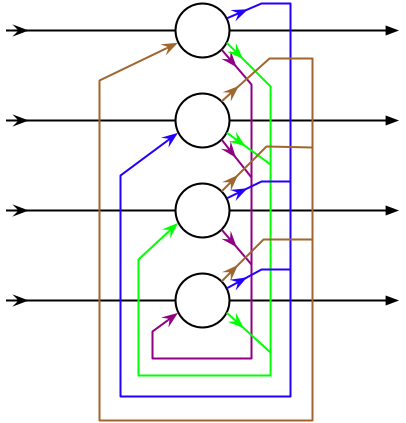
\includegraphics[width=\textwidth]{Images/Hopfield.png}
}\end{center}

\column{0.5\textwidth}
\uncover<+->{$$
\{X_1,\ldots,X_n\}
$$}

\uncover<+->{$$
W=\frac{1}{n}\sum_{i=1}^n X_i\times X_i^t
$$}
\end{columns}
\end{frame}

\begin{frame}\frametitle{Восстановление образа}
\begin{center}
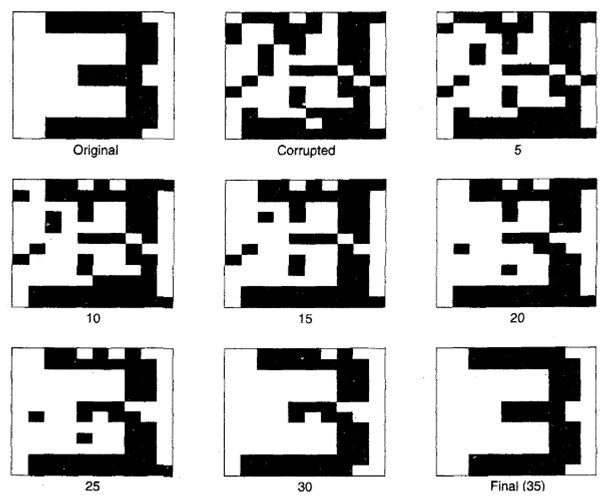
\includegraphics[width=0.8\textwidth]{Images/HopfieldSample.png}
\end{center}
\end{frame}

\begin{frame}\frametitle{Бинаправленная ассоциативная память}
\begin{columns}
\column{0.6\textwidth}
\begin{tikzpicture}[x=1.5cm]

	\foreach \num in {1,...,4}
	 	{
	 		\node[neu] (n-\num) at (2,4.5-\num) {};
	 		\node (y-\num) at (3,4.5-\num) {$y_{\num}$};
	 		\path (n-\num) edge (y-\num);
	 	}
	 \foreach \num in {1,...,5}
	 	{
	 	\node[neu] (m-\num) at (1,5-\num) {};
	 	\node (x-\num) at (0,5-\num) {$x_{\num}$};			
	 	\path (x-\num) edge (m-\num);
	 	}
	 	
\foreach \st in {1,...,4} \foreach \ds in {1,...,5} \path (n-\st) edge (m-\ds);
\end{tikzpicture}

\column{0.4\textwidth}
\uncover<+->{}
\uncover<+->{$$
X_i\rightarrow Y_i,\ i=1,\ldots,n
$$}
\uncover<+->{$$
W=\frac{1}{n}\sum_{i=1}^n X_i\times Y_i^t
$$}
\end{columns}
\end{frame}

\begin{frame}\frametitle{Восстановление образа}
\begin{columns}

\column{0.5\textwidth}
\uncover<+->{
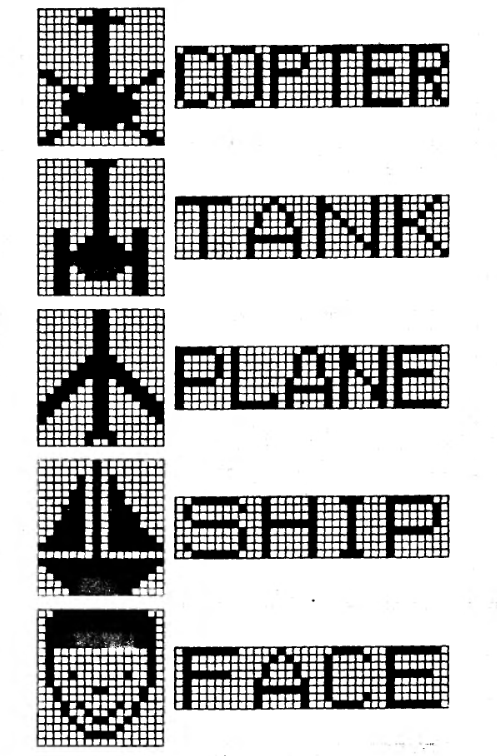
\includegraphics[width=\textwidth]{Images/BAMInput.png}
}
\column{0.5\textwidth}
\uncover<+->{
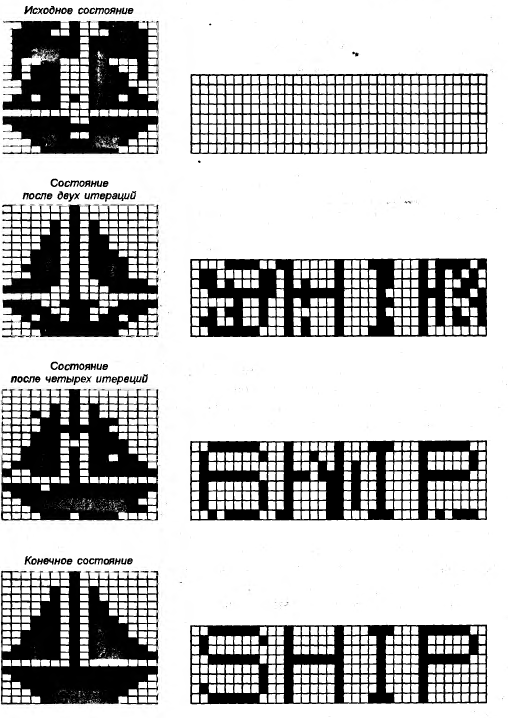
\includegraphics[width=\textwidth]{Images/BAMResult.png}
}
\end{columns}
\end{frame}

\begin{frame}
\doublebio
{Siegelmann}{Hava Siegelmann}
{Sontag}{Eduardo Sontag}
{
Computation Beyond the Turing Limit (1995)
}
\end{frame}

\begin{frame}\frametitle{Нейронная сеть с рациональными коэффициентами}

Для любой программы (т.е. машины Тьюринга) существует нейронная сеть с рациональными коэффициентами, вычисляющая ту же функцию.

\end{frame}

\begin{frame}\frametitle{Проблема останова}
\begin{itemize}
\item Не существует программы (т.е. машины Тьюринга) $P$, которая по тексту программы $X$ и ее входу $Y$ определяла, остановится ли $X$ на $Y$, или не остановится.
\item Не существует программы $P$, которая по тексту программы $X$ определяет, что она останавливается на любых входных данных.
\item Существует способ присвоить каждой программе уникальный целочисленный номер.
\item Пусть $M$ -- множество всех номеров, соответствующих программам, которые всегда останавливаются.
\item Тогда не существует программы, которая бы по числу $x$ проверяла, что $x\in M$
\end{itemize}
\end{frame}

\begin{frame}\frametitle{Нейронная сеть с действительными коэффициентами}



\begin{columns}



\column{0.4\textwidth}

\uncover<+->{$$
M=\{x_1,x_2,\ldots,x_n,\ldots\}
$$}
\uncover<+->{$$
x_i<x_{i+1}
$$}
\uncover<+->{$$
q=0,\underbrace{1\ldots1}_{x_1}0\underbrace{1\ldots1}_{x_2}0\ldots_2
$$}
\uncover<+->{
\begin{tikzpicture}[x=2cm,y=-2cm]
\node (x) at (0,0) {x};
\node (one) at (0,1) {1};
\node[neu] (n) at (1,1) {e};
\path (one) edge[->] node[above]{$q$} (n);
\node[draw=black,rectangle, inner sep=10] (p) at (2,0.5) {P};
\draw[->] (x) -| (p);
\draw[->] (n) -| (p);
\end{tikzpicture}
}

\column{0.6\textwidth}

\tikzstyle{block}=[draw=black,rectangle]
\tikzstyle{if}=[draw=black,diamond,aspect=2]

\uncover<+->{
\begin{tikzpicture}[y=-1.5cm,x=1.5cm]
\node[block] (v1) at (0,0) {$c=0$};
\node[block] (v2) at (0,1) {$a=\lfloor 2q \rfloor; q=2q-a;$};
\node[if] (v3) at(0,2) {$a=0?$};
\node[block] (v4) at(1,3) {$c++$};
\node[if] (v5) at(-1,3) {$c\ge x?$};
\node[block] (v6) at(0,4) {STOP};

\draw[->] (v1) -- (v2);
\draw[->] (v2) -- (v3);

\draw[->] (v3.east) -| node[right]{no} (v4);
\draw[->] (v3.west) -| node[left]{yes} (v5);
\draw[->] (v5.east) -| node[right]{yes} (v6);
\draw[->] (v5.west) |- node[left] {no}(v1);
\draw[->] (v4.east) -- ($(v4.east)+(0.5,0)$) |- (v1);
\end{tikzpicture}
}

\end{columns}




\end{frame}


\end{document}